%\begin{figure}[tb]
\begin{figure}[!htb]
    \centering
    \subfloat[MC, $60$ mm $<r<$ 100 mm]{\label{subfig:Ks_fit_MC_3}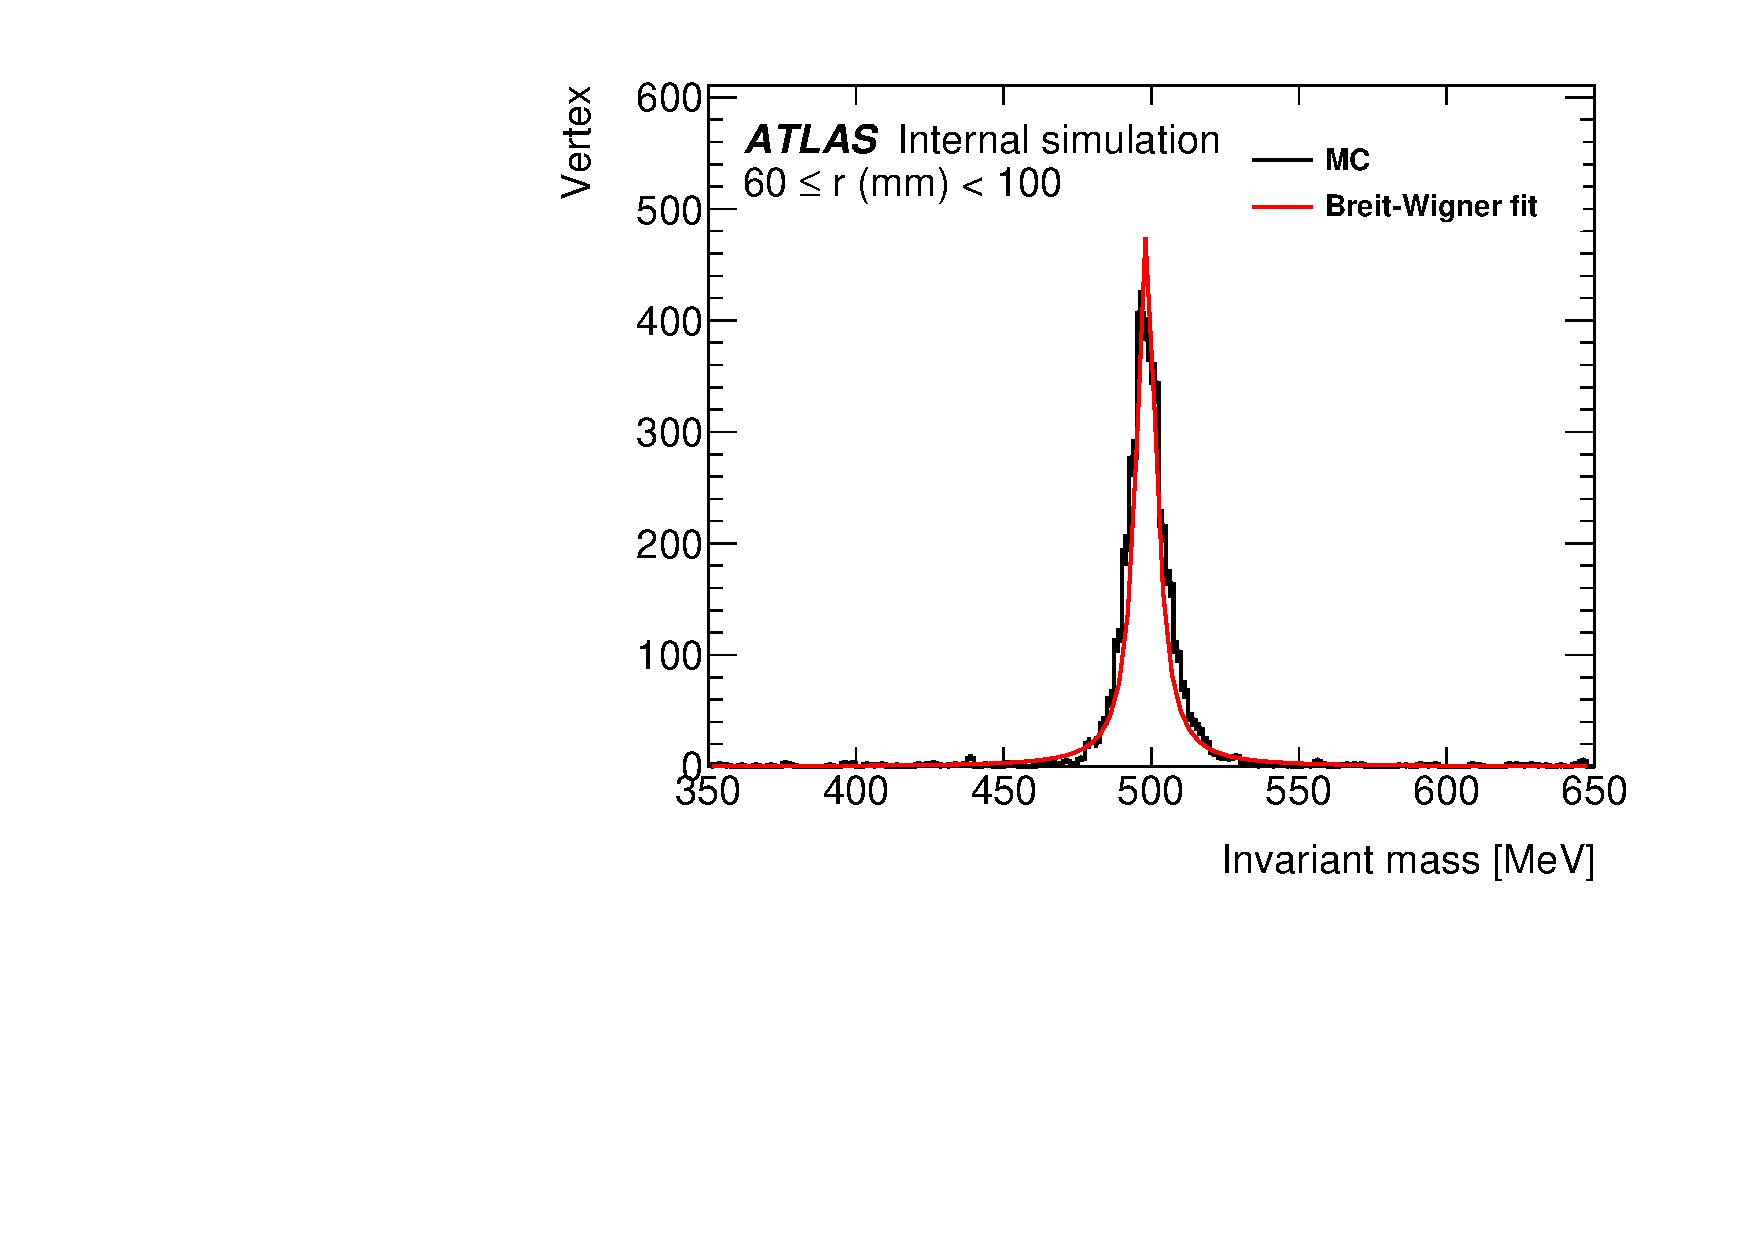
\includegraphics[width=0.33\textwidth]{figures/m_syst_Ks_Combined_MC_3}} 
    \subfloat[MC, $100$ mm $<r<$ 140 mm]{\label{subfig:Ks_fit_MC_4}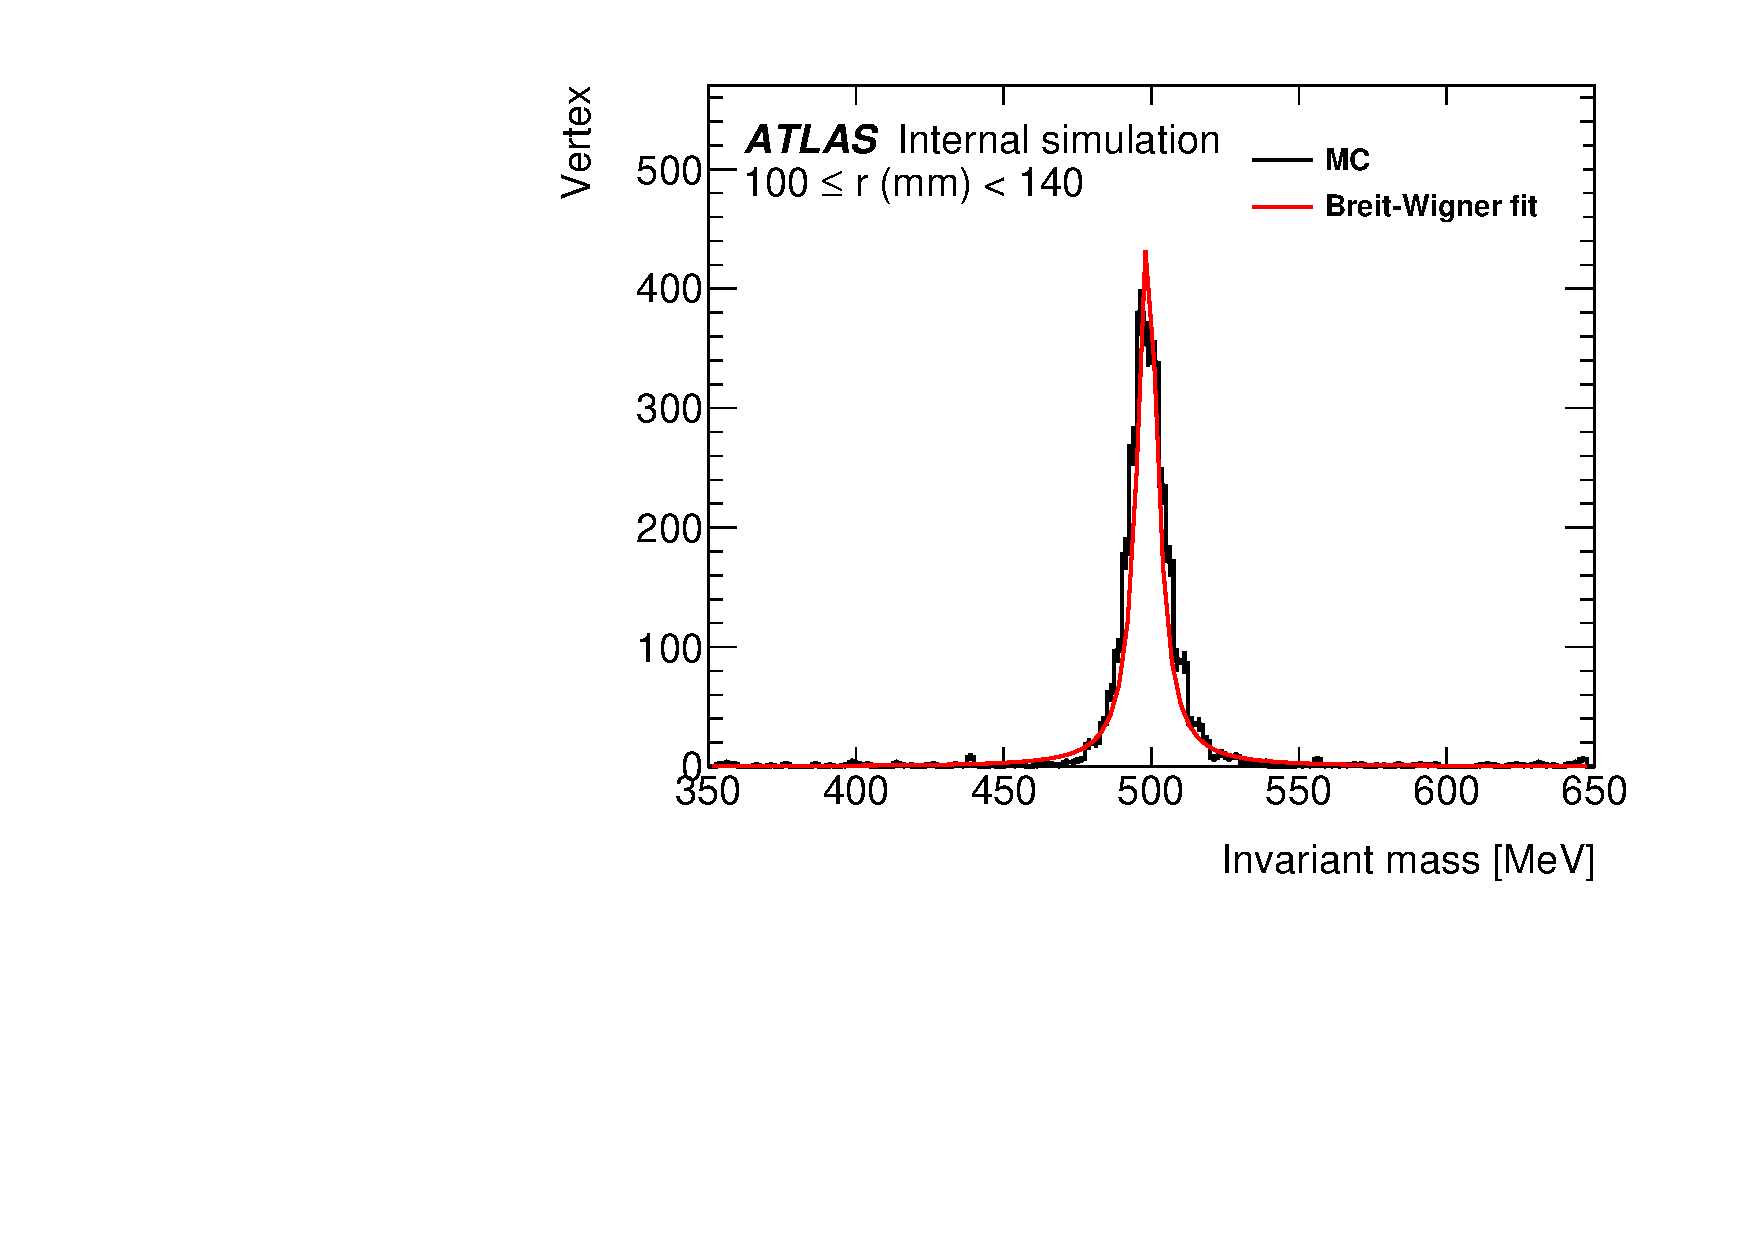
\includegraphics[width=0.33\textwidth]{figures/m_syst_Ks_Combined_MC_4}}
    \subfloat[MC, $140$ mm $<r<$ 180 mm]{\label{subfig:Ks_fit_MC_5}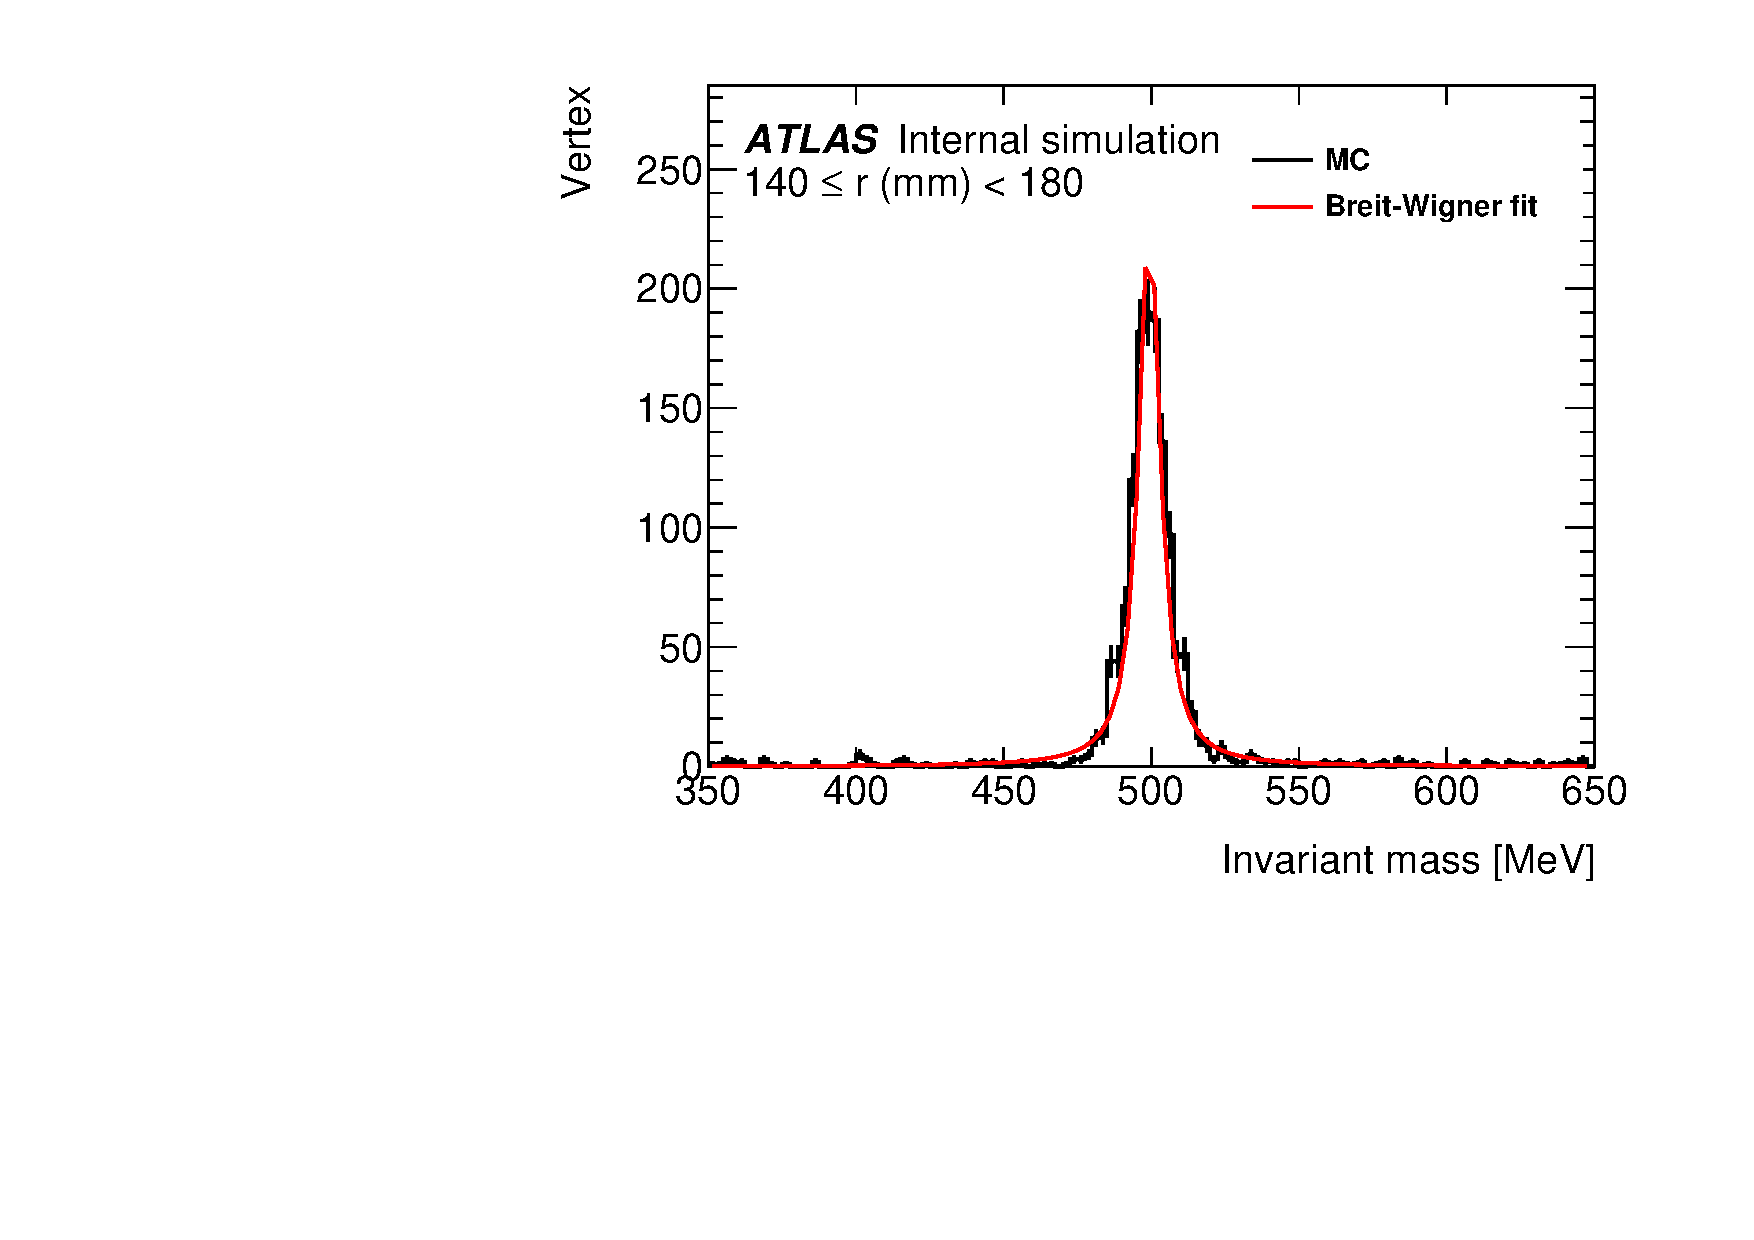
\includegraphics[width=0.33\textwidth]{figures/m_syst_Ks_Combined_MC_5}} \\
    \subfloat[MC, $180$ mm $<r<$ 220 mm]{\label{subfig:Ks_fit_MC_6}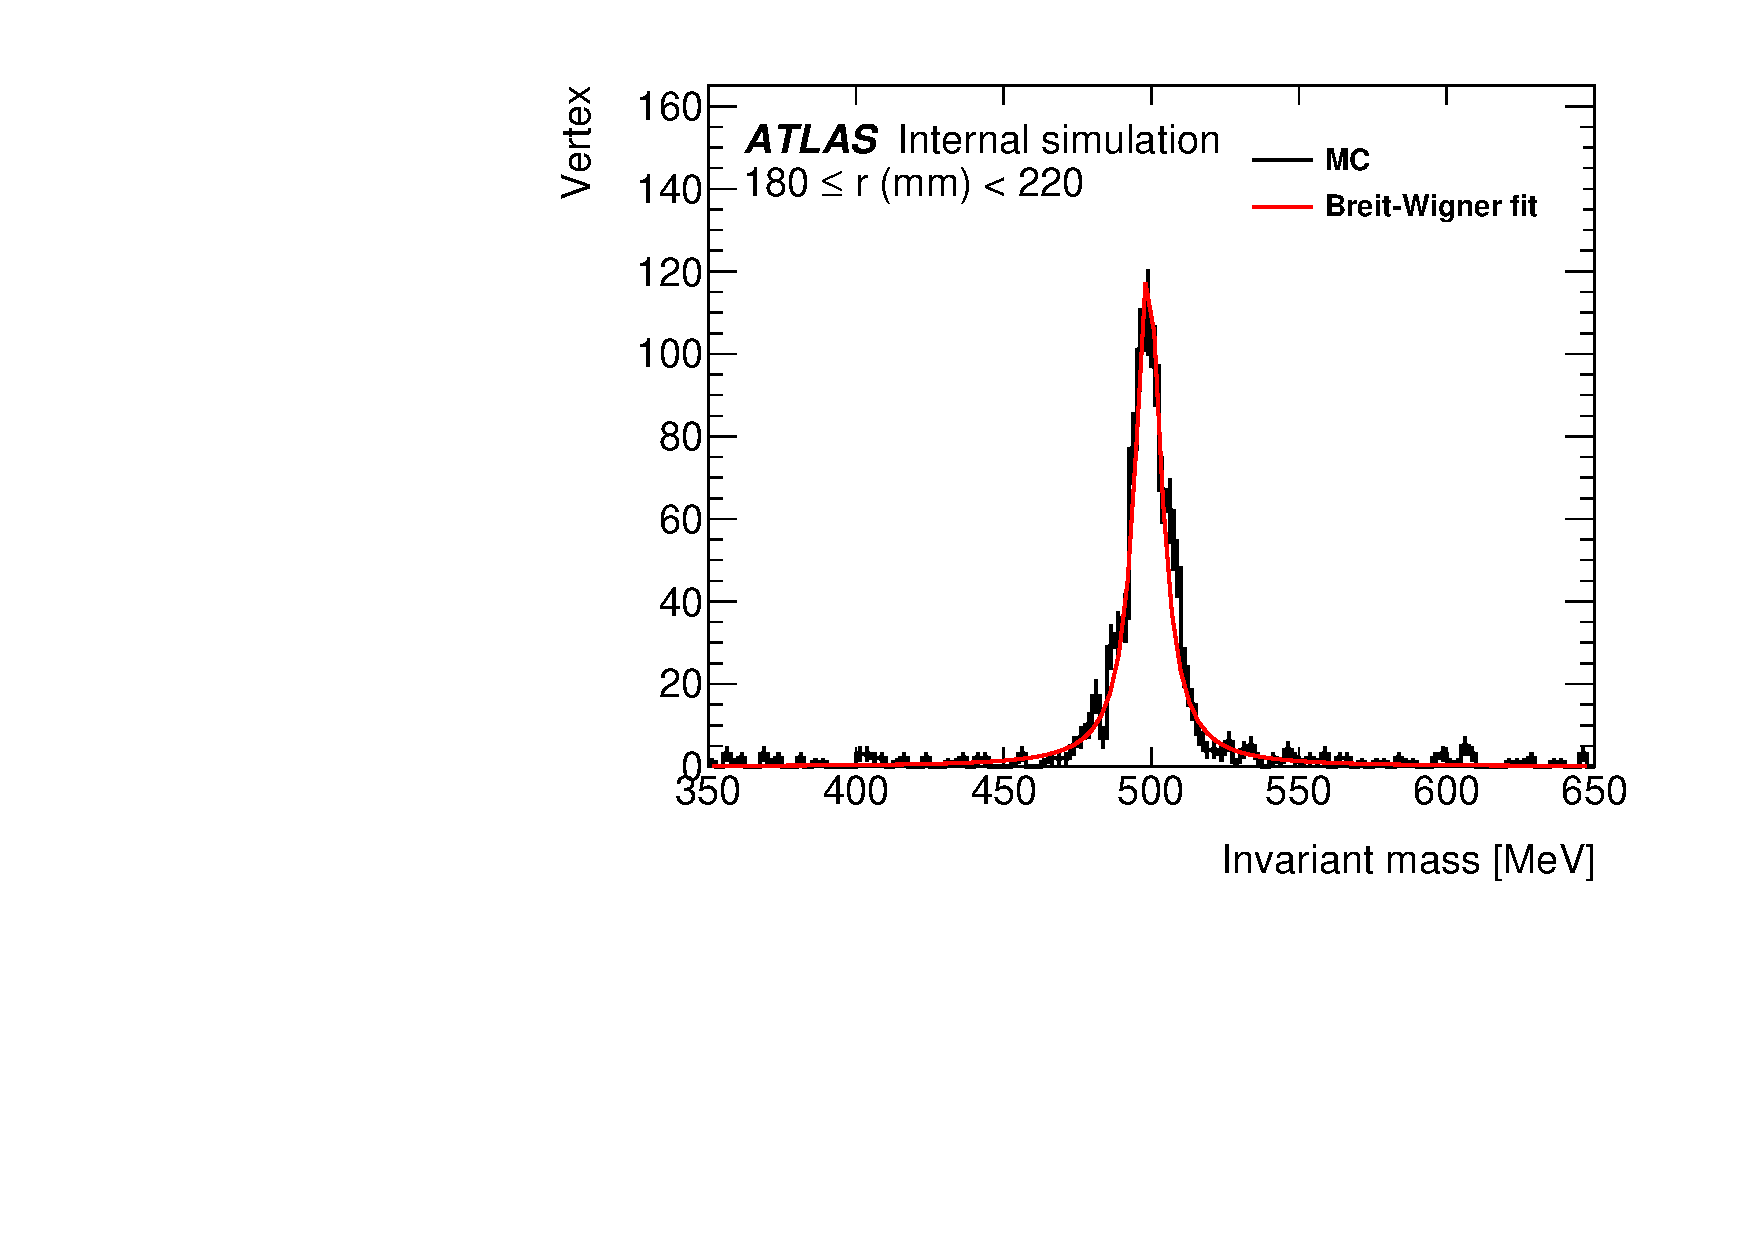
\includegraphics[width=0.33\textwidth]{figures/m_syst_Ks_Combined_MC_6}} 
    \subfloat[MC, $220$ mm $<r<$ 260 mm]{\label{subfig:Ks_fit_MC_7}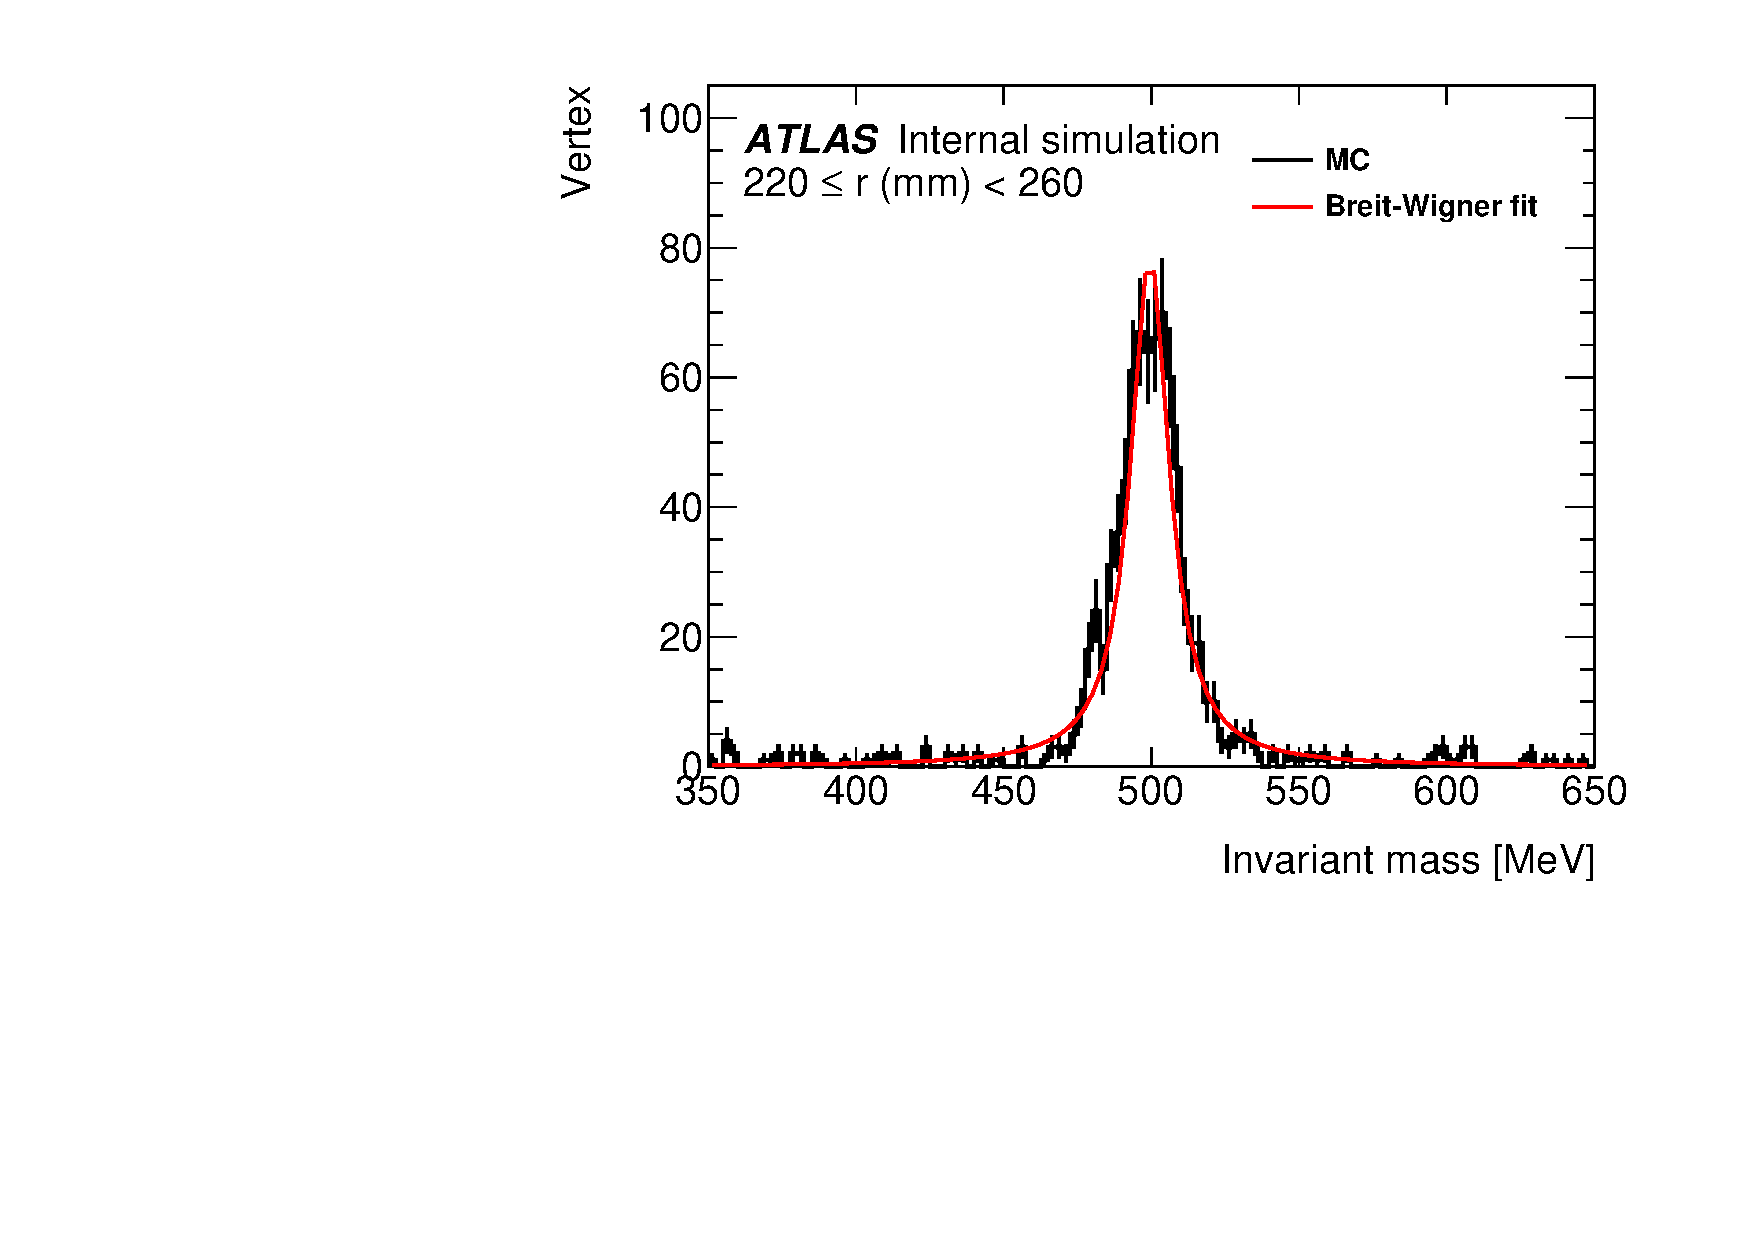
\includegraphics[width=0.33\textwidth]{figures/m_syst_Ks_Combined_MC_7}}
    \subfloat[MC, $260$ mm $<r<$ 300 mm]{\label{subfig:Ks_fit_MC_8}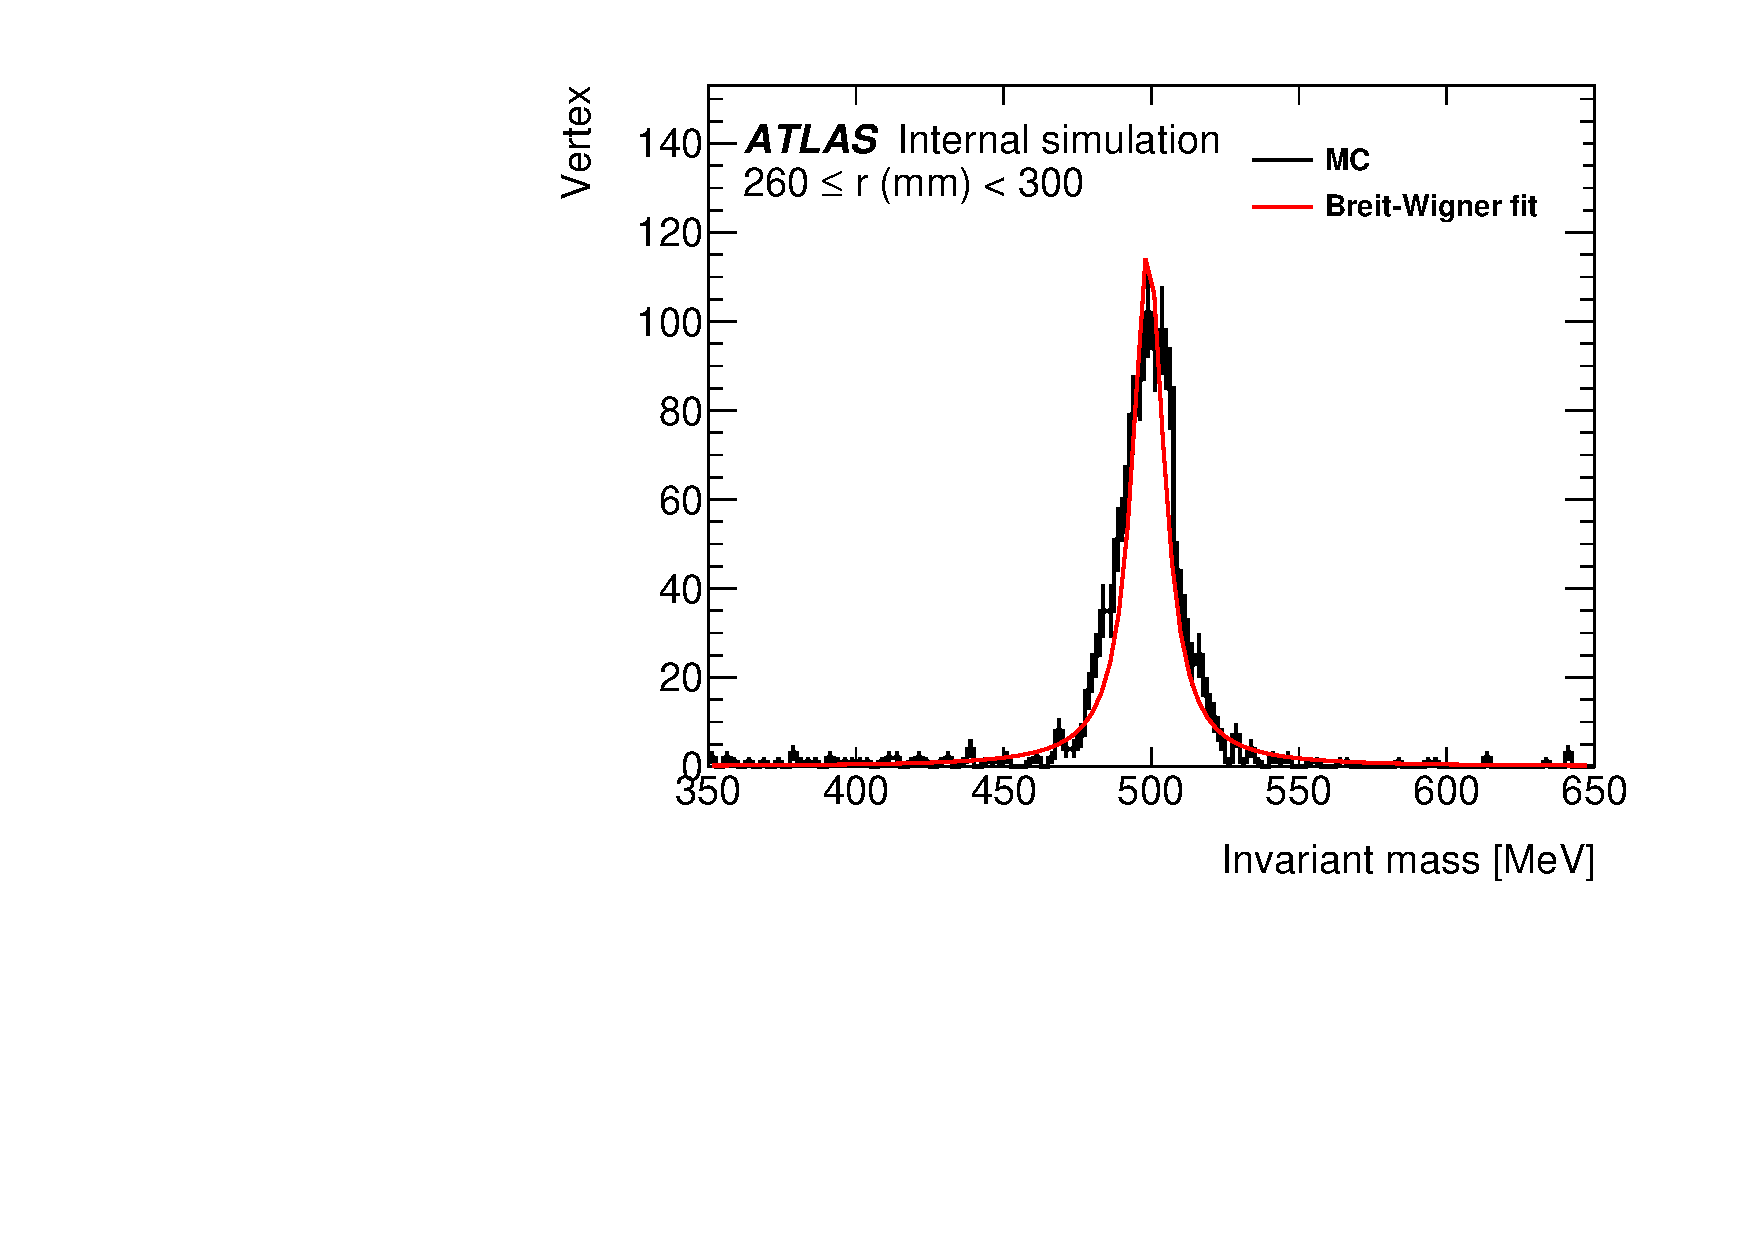
\includegraphics[width=0.33\textwidth]{figures/m_syst_Ks_Combined_MC_8}} \\
    \subfloat[Data, $r<20$ mm]{\label{subfig:Ks_fit_Data_1}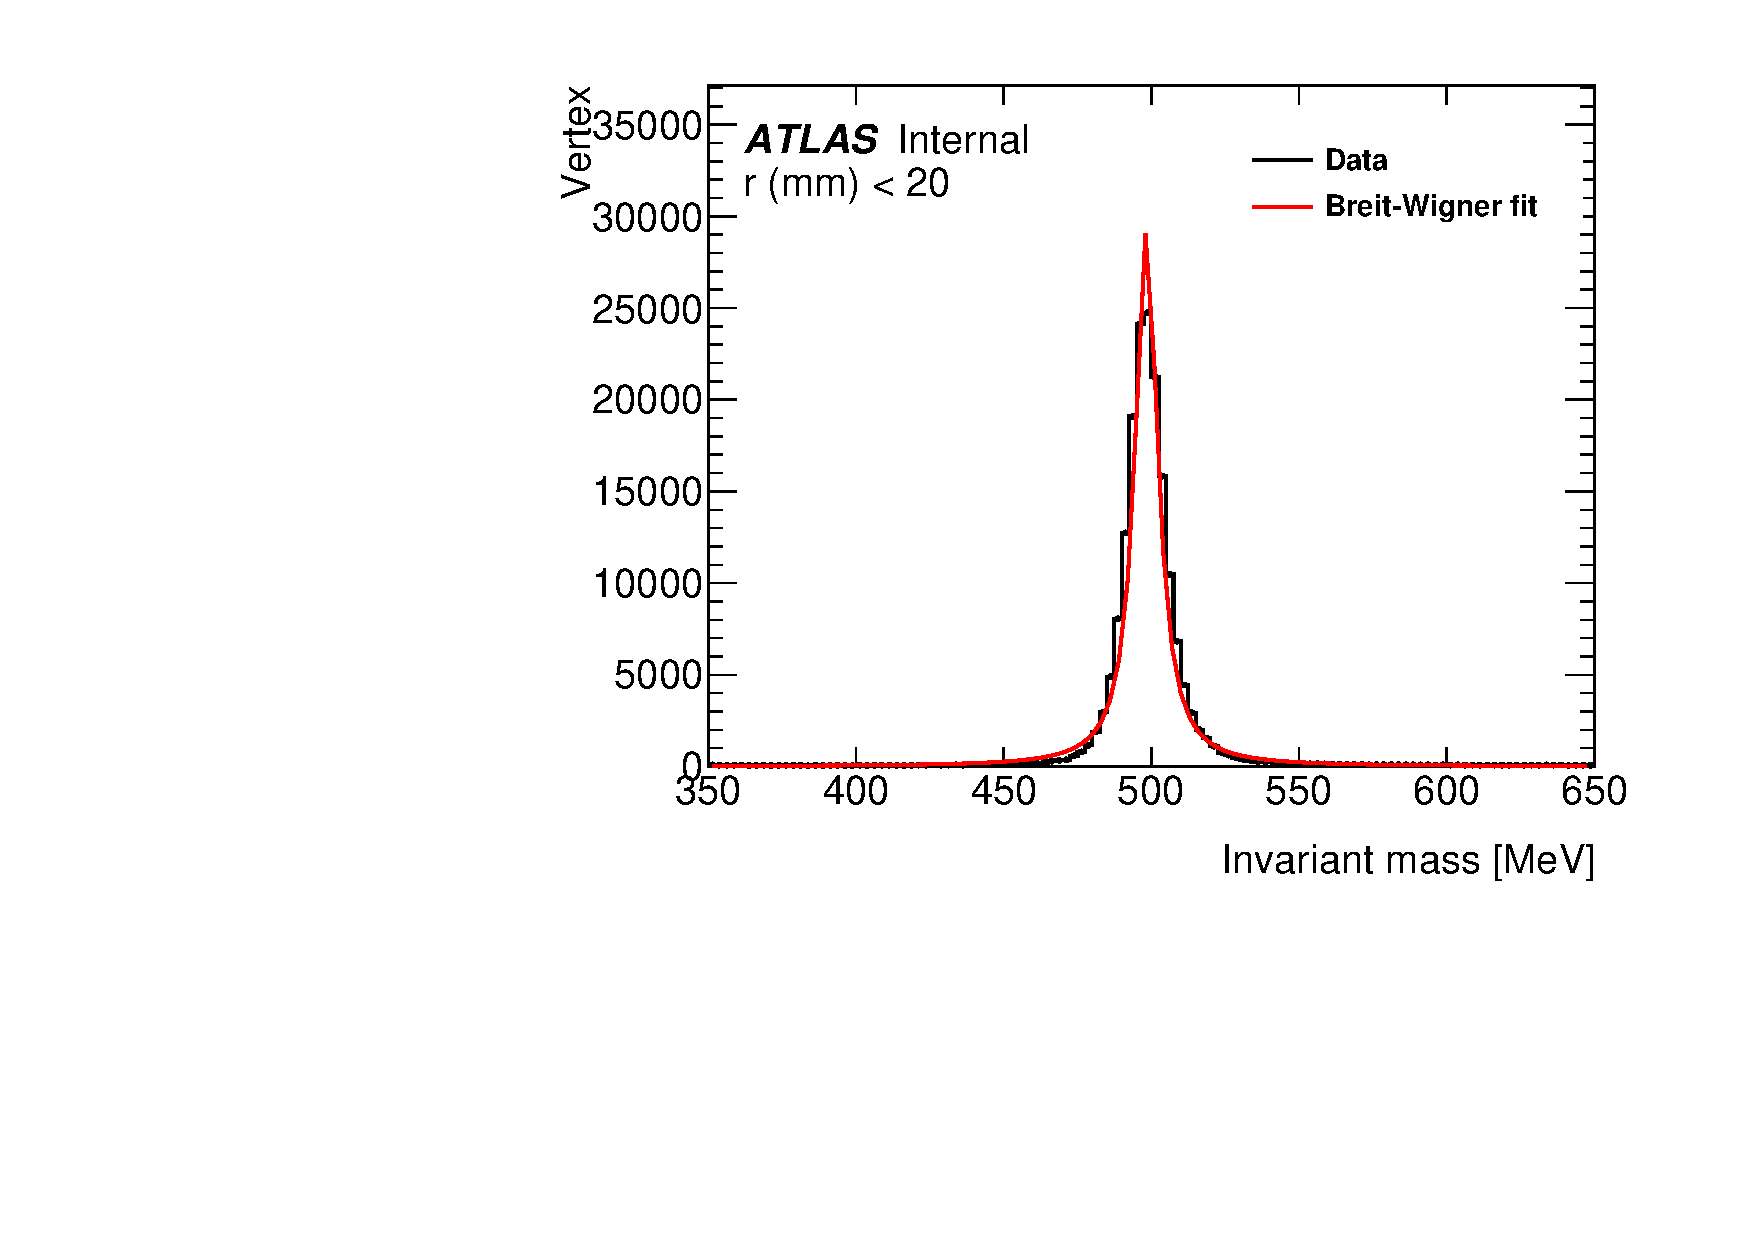
\includegraphics[width=0.33\textwidth]{figures/m_syst_Ks_Data_1}}
    \subfloat[Data, $100$ mm $<r<$ 140 mm]{\label{subfig:Ks_fit_Data_4}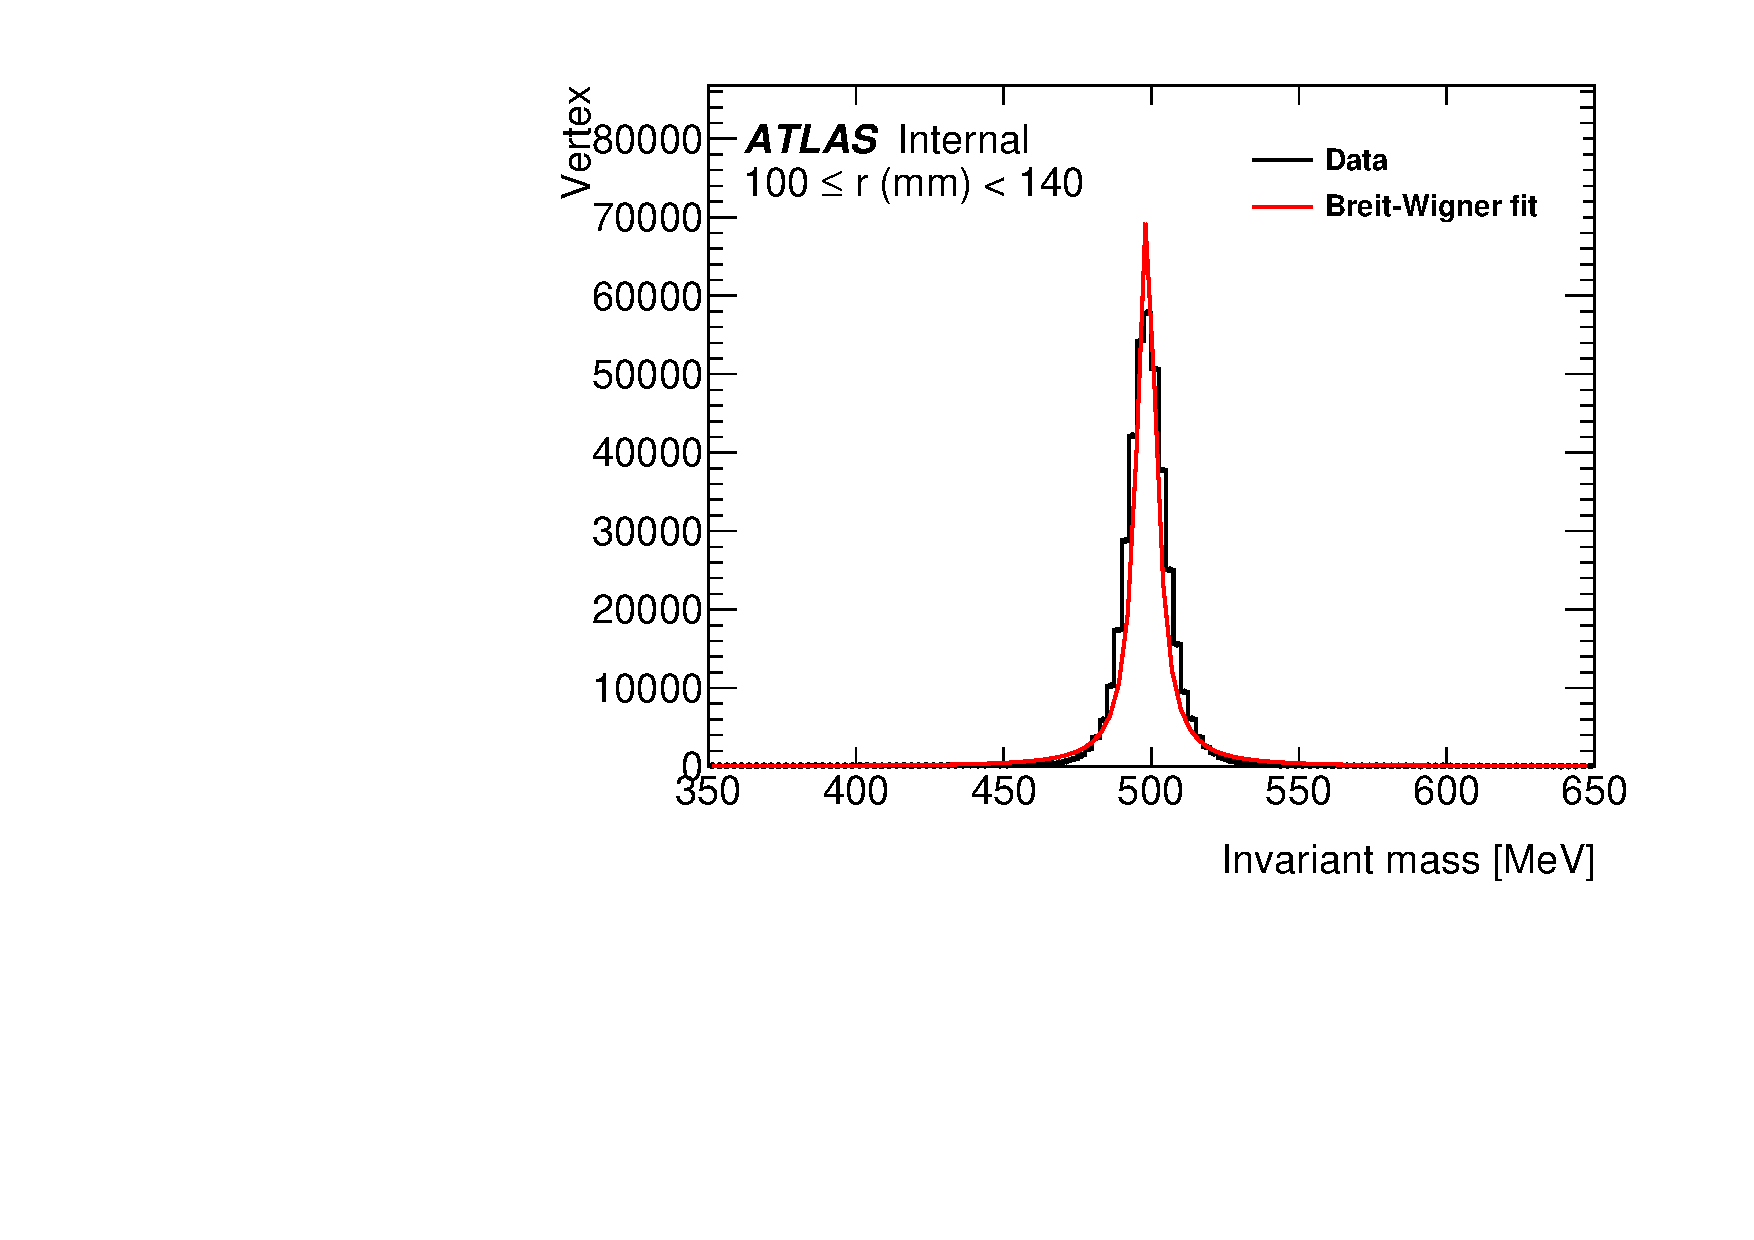
\includegraphics[width=0.33\textwidth]{figures/m_syst_Ks_Data_4}}
    \subfloat[Data, $140$ mm $<r<$ 180 mm]{\label{subfig:Ks_fit_Data_5}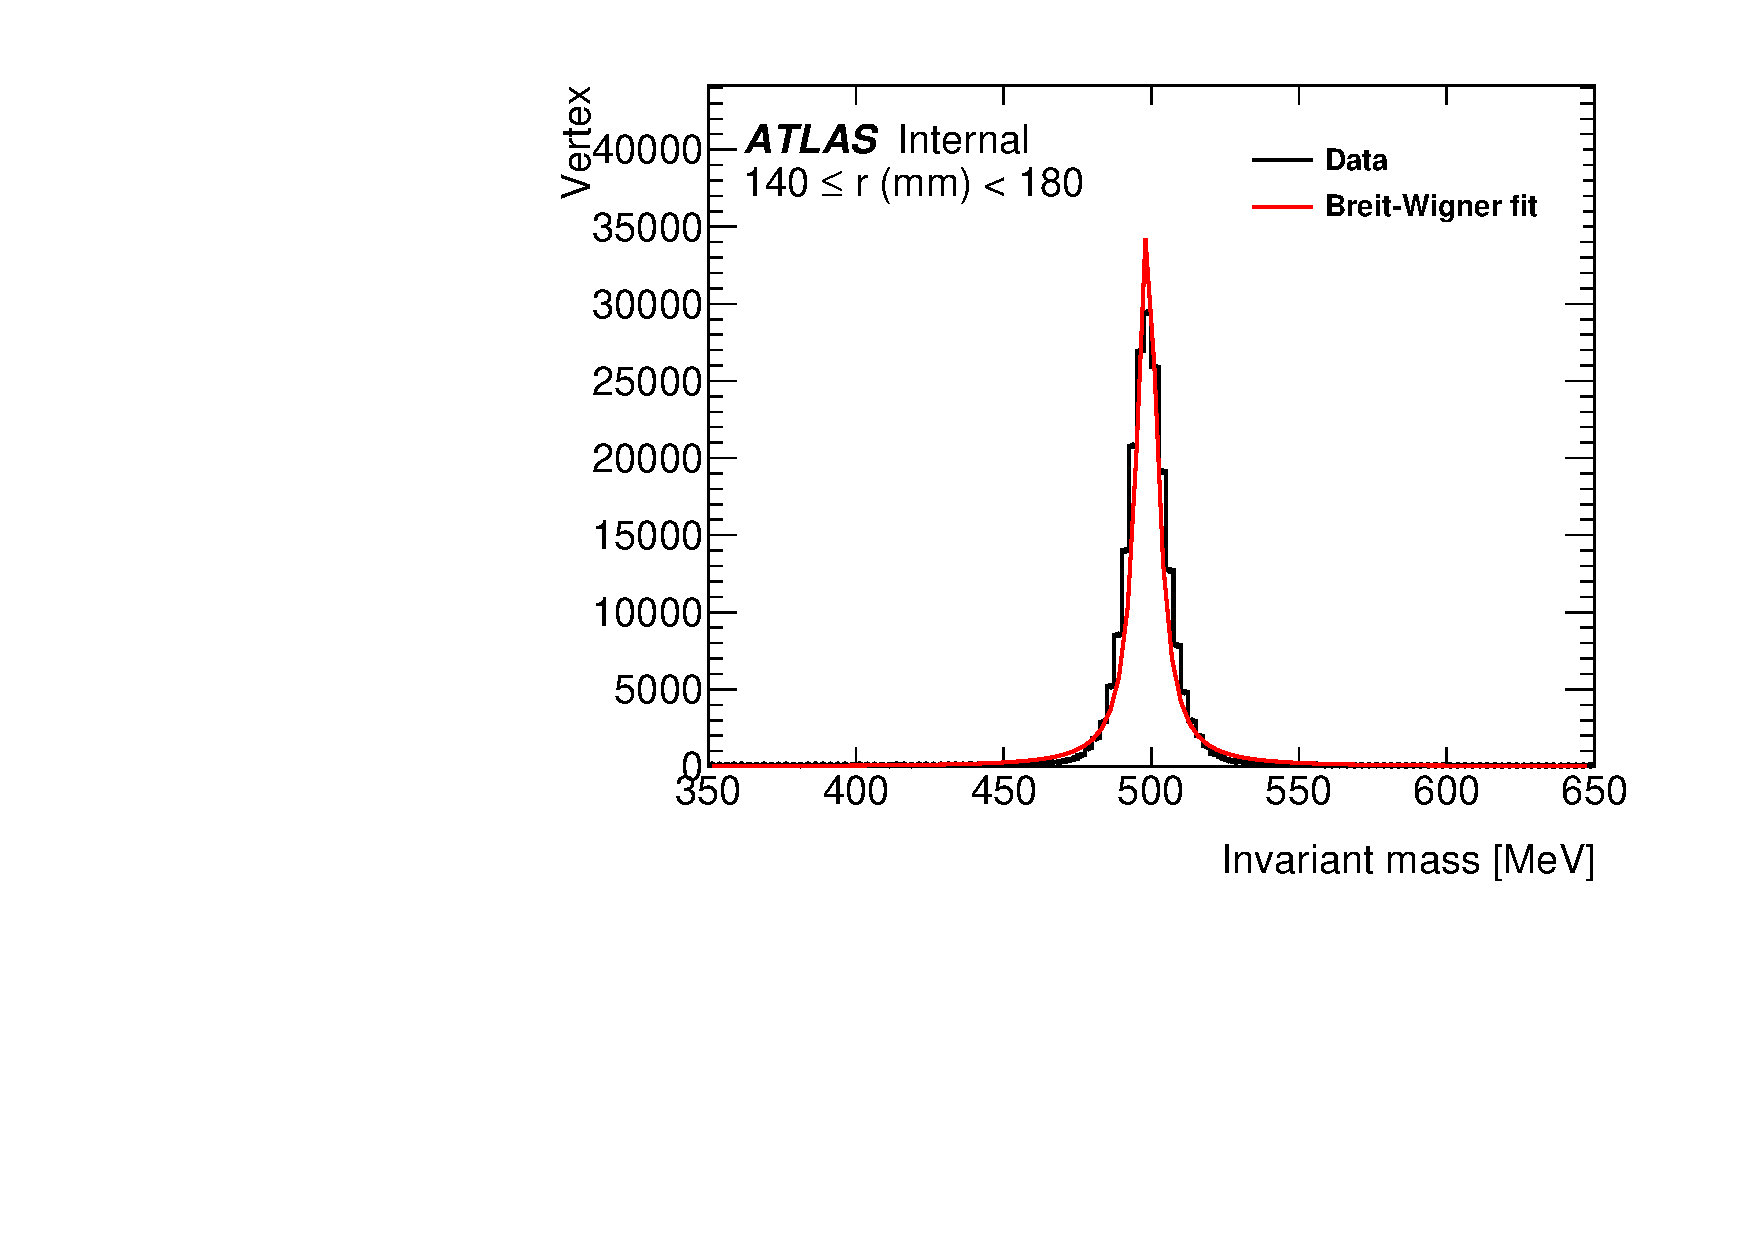
\includegraphics[width=0.33\textwidth]{figures/m_syst_Ks_Data_5}} \\
    \subfloat[Data, $180$ mm $<r<$ 220 mm]{\label{subfig:Ks_fit_Data_6}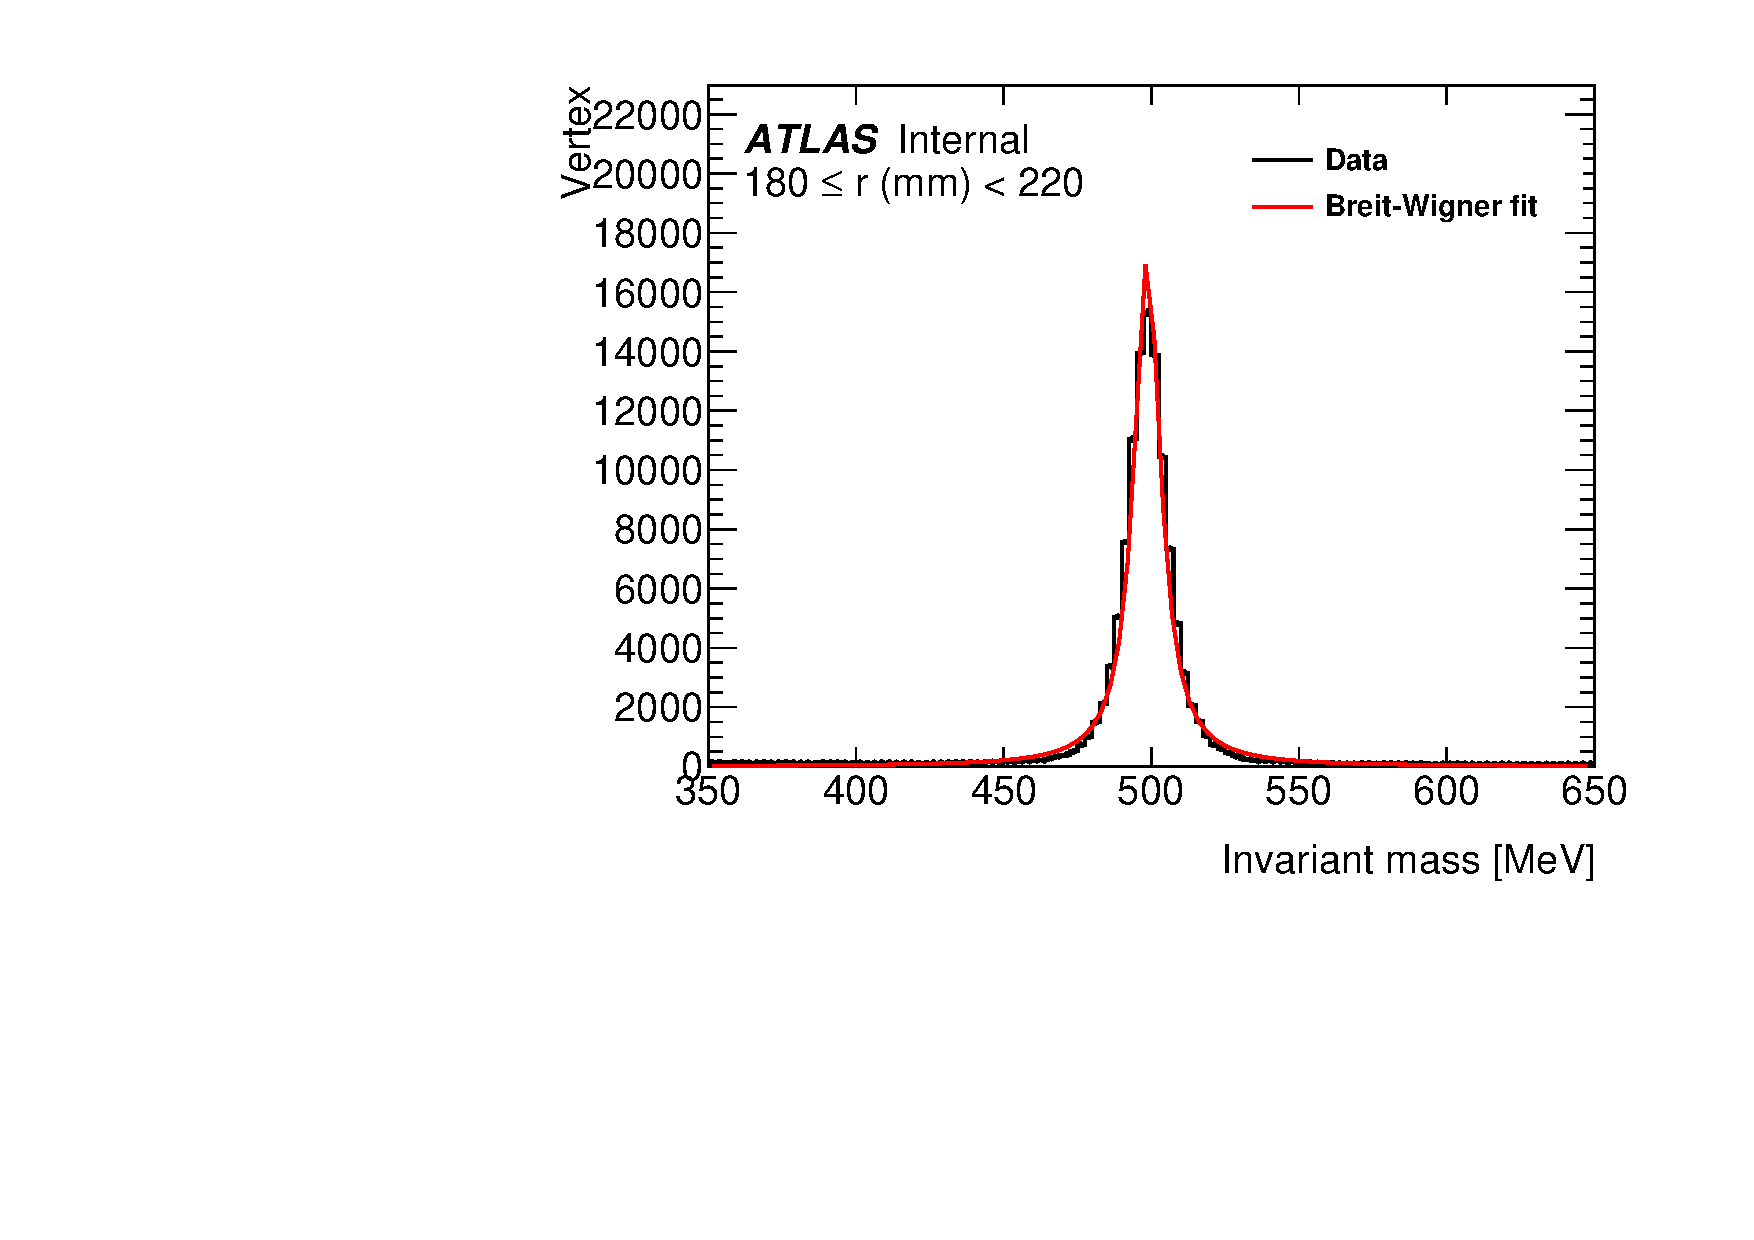
\includegraphics[width=0.33\textwidth]{figures/m_syst_Ks_Data_6}} 
    \subfloat[Data, $220$ mm $<r<$ 260 mm]{\label{subfig:Ks_fit_Data_7}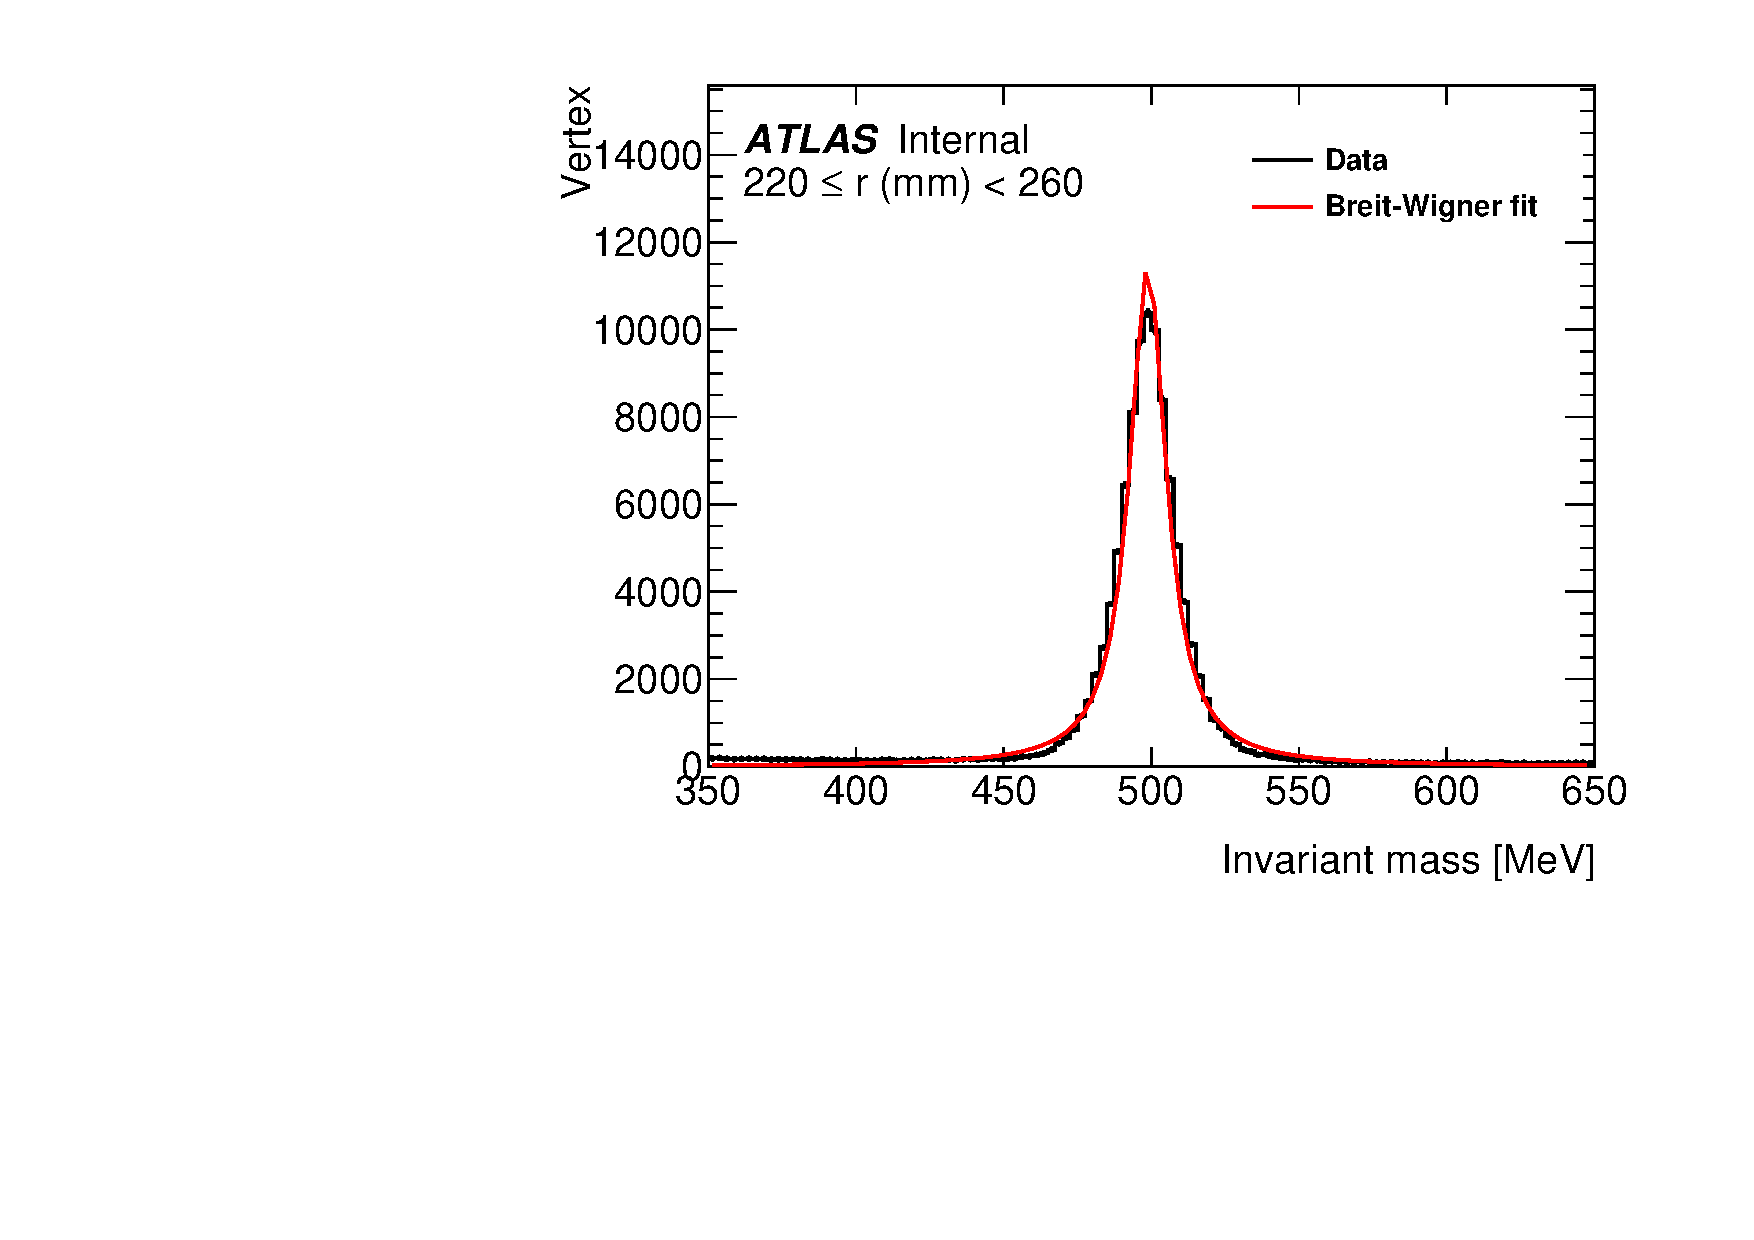
\includegraphics[width=0.33\textwidth]{figures/m_syst_Ks_Data_7}}
    \subfloat[Data, $260$ mm $<r<$ 300 mm]{\label{subfig:Ks_fit_Data_8}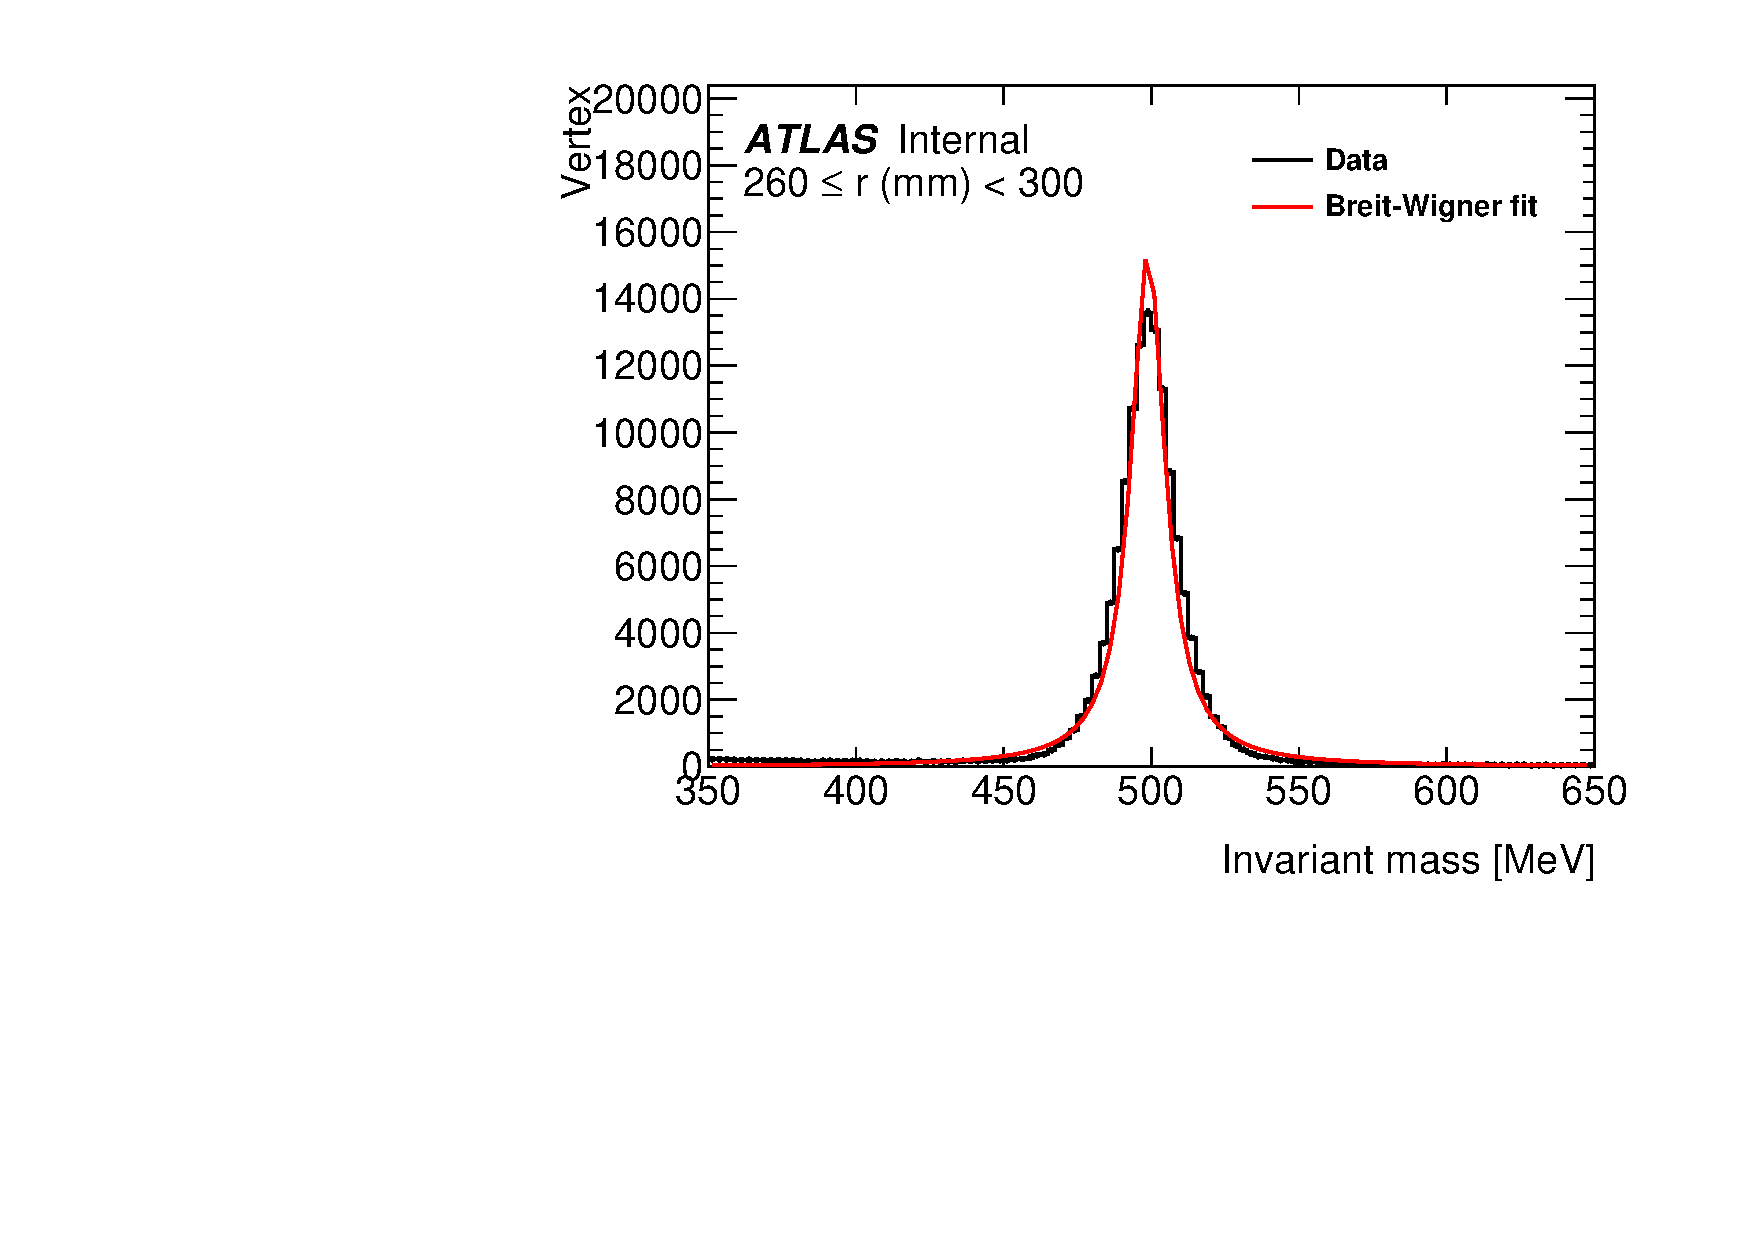
\includegraphics[width=0.33\textwidth]{figures/m_syst_Ks_Data_8}} \\
    \caption{$K_{S}$ invariant mass for various $r$. The curve shows a fit to Breit-Wigner.}
    \label{fig:Ks_fit_all}
\end{figure}



